\documentclass[doc_document.tex]{subfiles}
\begin{document}

\section{Style Transfer} \label{sec:style_transfer}


\begin{figure}
	\begin{center}
		\begin{tikzpicture}
		
		\node[rectangle, rounded corners, draw] (seg) {Segmentation};
		
		\node[inner sep=0pt, thick, black] (in) [left = of seg]
		{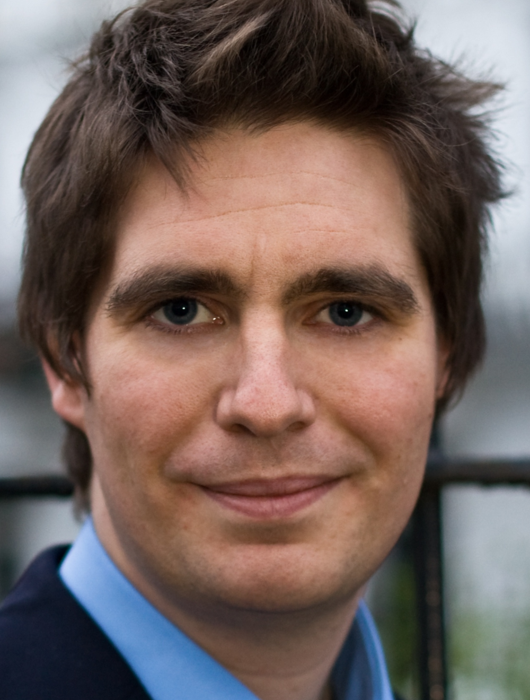
\includegraphics[width=.25\columnwidth,cfbox=black 1pt 1pt]{in11.png}};
			
		\node[inner sep=0pt, thick, black] (out) [right = of seg]
		{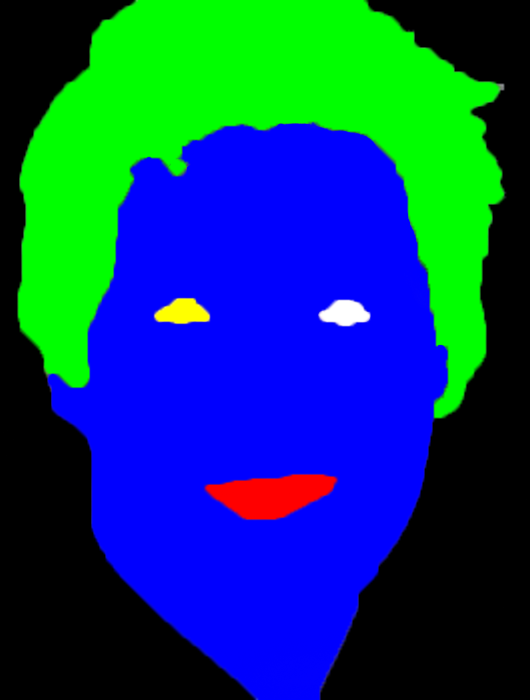
\includegraphics[width=.25\columnwidth,cfbox=black 1pt 1pt]{in11seg.png}};	
				
		\path [draw, ->, thick] (in) -- (seg);
		\path [draw, ->, thick] (seg) -- (out);
				
		\end{tikzpicture}
	\end{center}
	
	\caption{Segmentation of the content image} 
	\label{fig:segIn}
\end{figure}


\begin{figure}
	\begin{center}
		\begin{tikzpicture}
		
		\node[rectangle, rounded corners, draw] (seg) {Segmentation};
		
		\node[inner sep=0pt, thick, black] (in) [left = of seg]
		{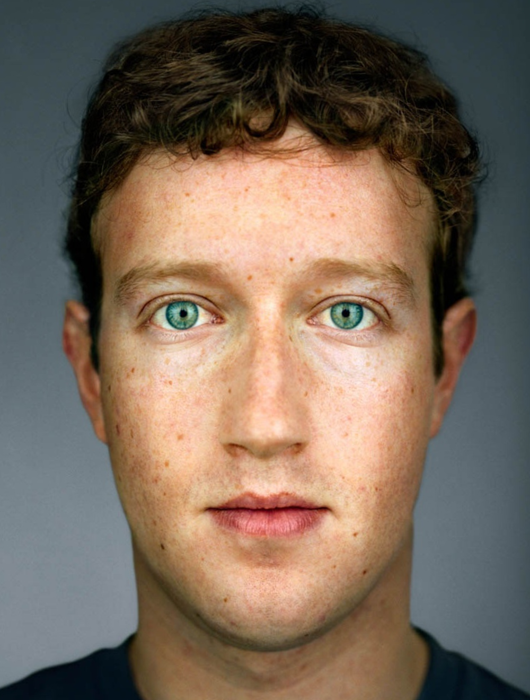
\includegraphics[width=.25\columnwidth,cfbox=black 1pt 1pt]{tar11.png}};
		
		\node[inner sep=0pt, thick, black] (out) [right = of seg]
		{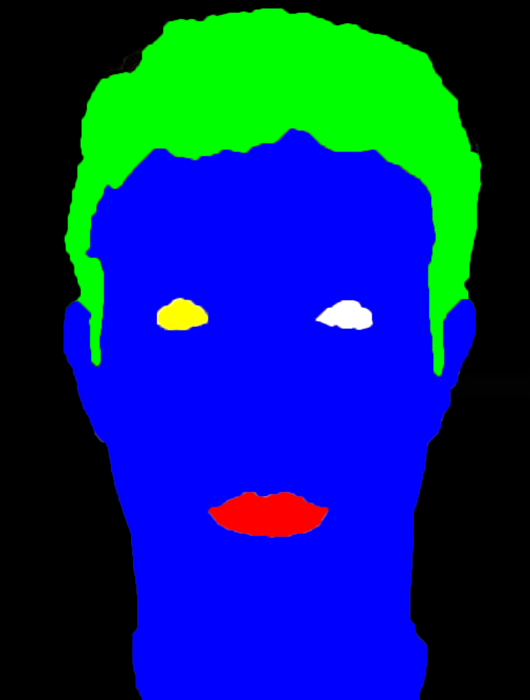
\includegraphics[width=.25\columnwidth,cfbox=black 1pt 1pt]{tar11seg.png}};	
		
		\path [draw, ->, thick] (in) -- (seg);
		\path [draw, ->, thick] (seg) -- (out);
		
		\end{tikzpicture}
	\end{center}
	
	\caption{Segmentation of the style image} 
	\label{fig:segTar}
\end{figure}

\begin{figure}
	\begin{center}
		\begin{tikzpicture}
		
		\node[rectangle, rounded corners, draw, align=center] (matting) {Closed-Form\\Matting};
		
		\node[inner sep=0pt, thick, black] (in) [left = of matting]
		{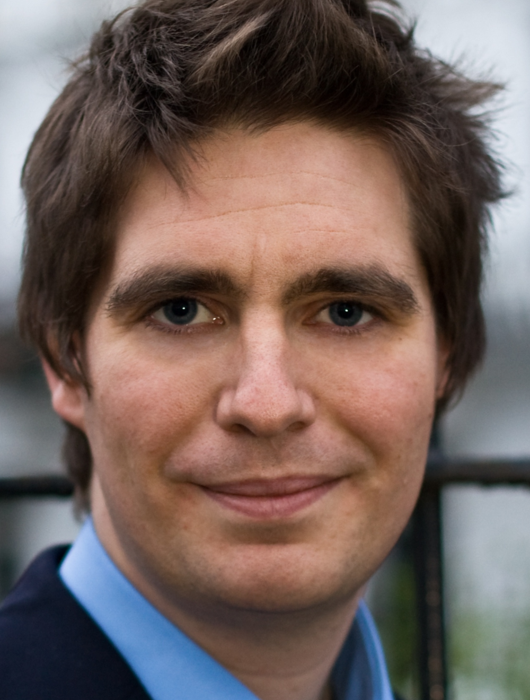
\includegraphics[width=.25\columnwidth,cfbox=black 1pt 1pt]{in11.png}};
		
		\node[rectangle, rounded corners, draw, align=center] (laplacian) [right = of matting] {Matting\\Laplacian};
				
		\path [draw, ->, thick] (in) -- (matting);
		\path [draw, ->, thick] (matting) -- (laplacian);
		
		\end{tikzpicture}
	\end{center}
	
	\caption{Closed-Form Matting with the content image} 
	\label{fig:matting}
\end{figure}

\begin{figure}
	\begin{center}
		\begin{tikzpicture}
		
		\node[rectangle, rounded corners, draw, align=center] (neuralStyle) {Neural Style\\Transfer};
		
		\node[inner sep=0pt, thick, black] (in) [left = of neuralStyle]
		{
\includegraphics[width=.25\columnwidth,cfbox=black 1pt 1pt]{noise.png}};
		
		\node[inner sep=0pt, thick, black] (out) [right = of neuralStyle]
		{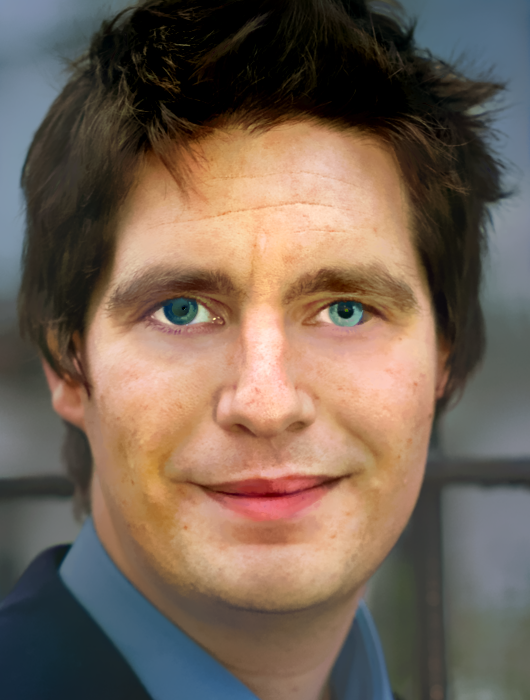
\includegraphics[width=.25\columnwidth,cfbox=black 1pt 1pt]{res11.png}};	
		
		\path [draw, ->, thick] (in) -- (neuralStyle);
		\path [draw, ->, thick] (neuralStyle) -- (out);
		
		\end{tikzpicture}
	\end{center}
	
	\caption{Neural Style Transfer} 
	\label{fig:neuralStyle}
\end{figure}

\end{document}